\documentclass[10pt, conference, compsocconf]{IEEEtran}
\usepackage{xltxtra}
\usepackage{subfig}
\usepackage{booktabs}
\usepackage{amsmath}
\usepackage[numbers,sort&compress]{natbib}
\setmainfont{Times New Roman}

\begin{document}

\title{idock 3: Ultrafast Protein-Ligand Docking on GPU Cluster} % can use linebreaks \\ within to get better formatting as desired
\author
{
\IEEEauthorblockN
{
Hongjian Li, Kwong-Sak Leung and Man-Hon Wong
\IEEEauthorblockA
{
Department of Computer Science and Engineering, Chinese University of Hong Kong, Hong Kong, P.R. China\\
JackyLeeHongJian@Gmail.com
}
}
}
\maketitle

\begin{abstract}

Protein-ligand docking is a key computational method in the design of starting points for the drug discovery process. We are motivated by the desire to accelerate large-scale docking and have thus developed idock 3 to utilize the tremendous computational power of GPU clusters.

\end{abstract}

\begin{IEEEkeywords}

bioinformatics, chemoinformatics, drug discovery, protein-ligand docking, virtual screening, multithreading

\end{IEEEkeywords}

\section{Introduction}

Protein-ligand docking predicts the preferred conformation and binding affinity of a small ligand as non-covalently bound to the specific binding site of a protein. Docking can therefore be used not only to determine whether a ligand binds, but also to understand how it binds. The latter is subsequently important to improve the potency and selectivity of binding. To date, there are hundreds of docking programs \cite{493,922}. The AutoDock series \cite{597,596,595} is the most cited docking software in the research community, with over 5,000 citations according to Google Scholar. AutoDock has contributed to the discovery of several drugs, including the first clinically approved HIV integrase inhibitor \cite{1169}. Following its initial release, several parallel implementations were developed using either multithreading or computer cluster \cite{115,560,782}.

In 2009, AutoDock Vina \cite{595} was released. As the successor of AutoDock 4 \cite{596}, AutoDock Vina significantly improves the average accuracy of the binding mode predictions while running two orders of magnitude faster with multithreading \cite{595}. It was compared to AutoDock 4 on selecting active compounds against HIV protease, and was recommended for docking large molecules \cite{556}. Its functionality of semi-flexible protein docking by enabling flexibility of side-chain residues was evaluated on VEGFR-2 \cite{1084}. To further facilitate the usage of AutoDock Vina, auxiliary tools were subsequently developed, including a PyMOL \cite{1221} plugin for program settings and visualization \cite{609}, a bootable operating system for computer clusters \cite{773}, a console application for virtual screening on Windows \cite{1268}, and a GUI for virtual screening on Windows \cite{1250}.

In 2011, inspired by AutoDock Vina, we developed idock 1.0 \cite{1153}, a multithreaded virtual screening tool for flexible ligand docking. idock introduces plenty of innovations, such as caching receptor and grid maps in memory to permit efficient large-scale docking, revised numerical model for much faster energy approximation, capability of automatic detection and deactivation of inactive torsions for dimensionality reduction, utilization of our lightweight thread pool to parallelize grid map creation and reuse threads, utilization of the new C++11 programming features to avoid frequent memory reallocation, and accelerated parsers for both receptors and ligands. When benchmarked on docking 10,928 drug-like ligands against HIV reverse transcriptase, idock 1.0 achieved a speedup of 3.3 in terms of CPU time and a speedup of 7.5 in terms of elapsed time on average compared to AutoDock Vina, making idock one of the fastest docking software.

Having released idock, we kept receiving docking requests from our colleagues and collaborators. They are mostly biochemists and pharmacologists, outsourcing the docking research to us after discovering pharmaceutical protein targets for certain diseases of therapeutic interest. Consequently, we had to grab the protein structure, do format conversion, define search space, set up docking parameters, and keep running idock in batch for months. Tedious enough, all the above work was done manually, resulting in very low research productivity. In order to automate large-scale protein-ligand docking using our idock, we have therefore developed a web platform called istar.

\section{Motivation}

Even though idock 2.0 outperformed AutoDock Vina \citep{595} by at least 8.69 times and at most 37.51 times in terms of docking speed and was capable of docking 16 ligands per minute on a high performance machine, it is estimated to require about 312 days, i.e. nearly a year, to dock the complete 7,220,835 drug-like ligands from ZINC against a certain protein, not to mention multiple proteins. Virtual screening remains a time-consuming practice. Faster implementations are highly desired.

We used AMD CodeAnalyst Performance Analyzer v3.6 to detect program hotspots and observe thread behaviors. Figure \ref{idock:ThreadProfile} shows the thread profile of idock. Thread 1060 was the main thread, while the other four were workers threads spawned by the main thread and maintained by our novel thread pool. During program startup, the main thread parsed command line arguments, initialized necessary variables, parsed receptor file, and created a thread pool to precalculate the scoring function in parallel. Afterwards, it entered a loop, docking ligands one by one. The four workers threads actually carried out the creation of grid maps as well as running Monte Carlo tasks in parallel, fully occupying all the four CPU cores. Upon completion of docking a ligand, program control was returned to the main thread to write conformations to file and read the next ligand from file. From the figure, it can be concluded that the worker threads acquire most of the CPU computing resources and the precalculation of grid maps and the execution of Monte Carlo tasks constitute the program hotspots, albeit the CPU-intensive Monte Carlo tasks and the I/O-intensive file reading/writing can be possibly pipelined according to our in-house trial.

\begin{figure}
\centering
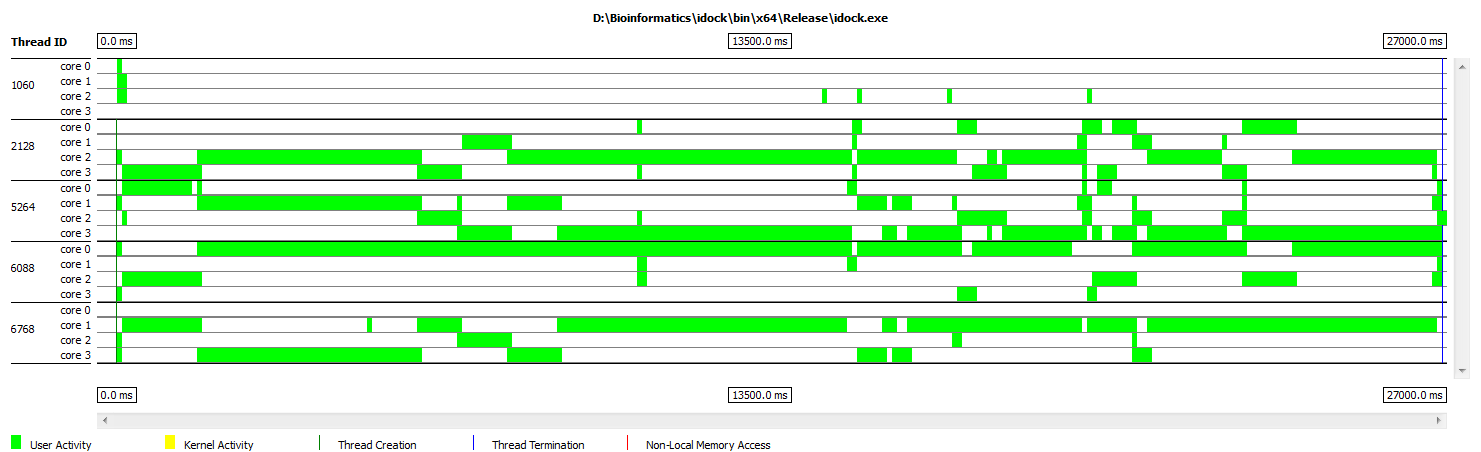
\includegraphics[width=\textwidth]{../idock3/ThreadProfile.png}
\caption{idock thread profile.}
\label{idock:ThreadProfile}
\end{figure}

We propose idock 3.0, incorporating GPU acceleration with both CUDA and OpenCL, harnessing the tremendous computational power and memory bandwidth offered by modern GPUs nowadays. In \citeyear{1138} we developed a fast CUDA implementation of agrep algorithm for approximate nucleotide sequence matching \citep{1138}, demonstrating our expertise in CUDA programming. Meanwhile, we are eagerly learning OpenCL. We will first work on a CUDA version, followed by an OpenCL version.

\section{Methods}

idock 3 is written in C++11 with CUDA driver API. Low level. Forward compatibility.

Performance optimization revolves around three basic strategies: 1) maximizing parallel execution, 2) maximizing memory bandwidth, and 3) maximizing instruction throughput.

Maximizing parallel execution can be achieved by exposing as much data parallelism as possible and mapping the parallelism to the hardware as efficiently as possible. In dock, we have parallelized both the precalculation of grid maps and the Monte Carlo global optimization using our novel thread pool in order to thoroughly utilize multicore CPU. We plan to port these two most time-consuming parts to the GPU, map Monte Carlo tasks directly to CUDA threads, and use NVIDIA's occupancy calculator to carefully choose the execution configuration of each kernel launch in order to maintain a high GPU utilization. Several technical difficulties exist. One difficulty is the lack of sufficient capacity of GDDR5 memory, which is merely 2GB along with a GeForce GTX 680. This restriction voids the precalculation of grid maps at a fine granularity like 0.08\AA, leading to reduced approximation accuracy and possibly a high false negative rate. Another difficulty is the efficient generation of pseudo random numbers. Although there are official libraries and third-party libraries to facilitate this purpose, it is hard to determine the number of random numbers in need in advance because the Monte Carlo algorithm is stochastic \textit{per se}.

Maximizing memory bandwidth can be achieved by minimizing data transfers between the CPU and the GPU and optimizing the access patterns to global memory and shared memory on the GPU. Since CPU-to-GPU and GPU-to-CPU data transfers have much lower bandwidth than internal GPU data transfers, we plan to accommodate as much data as possible into the GPU global memory. In idock 3.0, constant data such as structure of receptor, definition of search space, precalculation of scoring function, and configurations for the BFGS Quasi-Newton local optimizer will reside in constant cache, while grid maps, due to its huge size, will reside in global memory, and temporary variables will reside in per-thread registers.

Maximizing global memory bandwidth is of crucial importance, and its bandwidth depends largely on its access pattern. Figure \ref{GPU:AlignedSequentialGlobalMemoryAccess} shows an example of aligned and sequential global memory access and corresponding memory transactions based on compute capability. In this case, 32 threads of a warp access adjacent 4-byte words such as adjacent single precision float values or 32-bit integer values. In other words, the \textit{k}th thread accesses the \textit{k}th 4-byte word in a 128B L1 cache line, a single coalesced transaction alone will service that memory access. In idock 3.0, we will adopt this kind of aligned and sequential access pattern and re-organize array of structures into structure of arrays, e.g.  [ \{ x1, y1, z1 \}, \{ x2, y2, z2 \} ] into \{ [ x1, x2 ], [ y1, y2 ], [ z1, z2 ] \}. Such a restructuring requires rewriting almost all the relevant mathematical data structures and functions in use in idock. So far we have stepped towards this direction a little bit, finishing rewriting the template class of quaternion from the BOOST C++ library into our own lightweight version to represent the orientation of a conformation.

\begin{figure}
\centering
%\includegraphics[width=\linewidth]{../idock3/AlignedSequentialGlobalMemoryAccess.png}
\caption{Aligned and sequential global memory accesses by a warp, 4-byte word per thread, and associated memory transactions based on compute capability. Source: NVIDIA.}
\label{GPU:AlignedSequentialGlobalMemoryAccess}
\end{figure}

A GK104 SMX has 64KB of on-chip memory that can be configured as 48KB of shared memory with 16KB of L1 cache, or as 16KB of shared memory with 48KB of L1 cache. Since threads within a thread block run their Monte Carlo tasks independently and seldom communicate with one another, we decide to allocate 48KB of the 64KB on-chip memory to L1 cache.

Maximizing instruction throughput can be achieved by using single precision floating point instead of double precision and using intrinsics instead of regular functions. This strategy suggests trading precision for speed as long as the final result is not affected. Since most contemporary GPU chips supply with an astonishingly high throughput for single precision operations at TFLOP level but a relatively low throughput for double precision operations, we prefer the former. In order to make sure the precision loss must not affect the end result too much, we did an in-house trial, demoting double to float in idock, only to find that the predicted conformation and free energy were exactly identical as in the case of double precision given the same random seed for initializing the pseudo random number generator. This experiment concluded idock to be insensitive to precision switch and it is thus safe to utilize single precision operations as well as native intrinsics in idock 3.0.

\subsection{Scoring Function}
RF-Score

\subsection{Docking Algorithm}
BFGS

Vina, simulated annealing, CPU async execution

Monte Carlo
same PC in warp, less divergence
greedy, no metropolis acceptance
mutate current local optimum

Monte Carlo
mutate so-far-best local optimum

\subsection{CUDA Kernel Design}

Address Spaces
global, constant, shared, local
Data Structures
AOS to SOA to meet requirements of global memory coalesced access.

\subsection{Scheduling Models}

In Vina, threads are created just in time. Suffer from thread construction and destruction overhead.

In idock 2.0, a lightweight thread pool, to reuse threads.

In idock 3.0, 
Central dispatcher, multiple devices as concurrent consumers, each has a command queue
device queue size = 1, main thread syncs with device before fetching next task
Overlap host threads with device threads
Thread construction and destruction overhead is one off.

HyperQ on compute capability 3.5 and higher, and Souther Islands
Parallel compute and transfer, applied to CPU too
device queue size > 1

\section{Results and Discussion}

\subsection{Strong Scaling}



\subsection{Weak Scaling}

\subsection{Impact of simulation Runs on Docking Accuracy}

\subsection{HyperQ Speedup}


\section{Availability}

idock is free and open source under Apache License 2.0. Its precompiled executables for 64-bit Linux and Windows, docking examples and API documentations are available at https://GitHub.com/HongjianLi/idock. A web server for large-scale protein-ligand docking is available at http://istar.cse.cuhk.edu.hk/idock.

\section{Conclusion}

We shall be able to do two things that are not possible at present. One one hand, we shall fine tune the parameters of our BFGS local optimizer in order to increase the redocking success rate. Those parameters include the early stopping criterion, the step size in line search, the apprximation of inverse Hessian matrix, and so on. On the other hand, we shall perform proteomic-scale docking for the entire solved proteins in PDB \citep{540,537} and warehouse the huge results into a public database. We believe the community will definitely benefit from such a database with pre-docked information instantly available.

\section{Acknowledgements}
This work is supported by EGC.

\bibliographystyle{unsrtnat}
\bibliography{refworks}

\end{document}
